\documentclass[conference]{IEEEtran}
\IEEEoverridecommandlockouts
% The preceding line is only needed to identify funding in the first footnote. If that is unneeded, please comment it out.
\usepackage{cite}
\usepackage{amsmath,amssymb,amsfonts}
\usepackage{algorithmic}
\usepackage{graphicx}
\usepackage{textcomp}
\usepackage{xcolor}
\usepackage{subfigure}
\usepackage[numbers]{natbib}

%\usepackage{ulem}
\usepackage{url}
\usepackage{tabu}
\usepackage[numbers]{natbib}
\citestyle{IEEEtran}
\bibliographystyle{IEEEtranN}


%\def\BibTeX{{\rm B\kern-.05em{\sc i\kern-.025em b}\kern-.08em
%    T\kern-.1667em\lower.7ex\hbox{E}\kern-.125emX}}
\begin{document}

\title{Blockchain Trading Graph Embedding*\\
{\footnotesize \textsuperscript{*}Note: Sub-titles are not captured in Xplore and
should not be used}
\thanks{Identify applicable funding agency here. If none, delete this.}
}

\author{\IEEEauthorblockN{1\textsuperscript{st} Given Name Surname}
\IEEEauthorblockA{\textit{dept. name of organization (of Aff.)} \\
\textit{name of organization (of Aff.)}\\
City, Country \\
email address}
\and
\IEEEauthorblockN{2\textsuperscript{nd} Given Name Surname}
\IEEEauthorblockA{\textit{dept. name of organization (of Aff.)} \\
\textit{name of organization (of Aff.)}\\
City, Country \\
email address}
\and
\IEEEauthorblockN{3\textsuperscript{rd} Given Name Surname}
\IEEEauthorblockA{\textit{dept. name of organization (of Aff.)} \\
\textit{name of organization (of Aff.)}\\
City, Country \\
email address}
\and
\IEEEauthorblockN{4\textsuperscript{th} Given Name Surname}
\IEEEauthorblockA{\textit{dept. name of organization (of Aff.)} \\
\textit{name of organization (of Aff.)}\\
City, Country \\
email address}
\and
\IEEEauthorblockN{5\textsuperscript{th} Given Name Surname}
\IEEEauthorblockA{\textit{dept. name of organization (of Aff.)} \\
\textit{name of organization (of Aff.)}\\
City, Country \\
email address}
\and
\IEEEauthorblockN{6\textsuperscript{th} Given Name Surname}
\IEEEauthorblockA{\textit{dept. name of organization (of Aff.)} \\
\textit{name of organization (of Aff.)}\\
City, Country \\
email address}
}

\maketitle

\begin{abstract}
This document is a model and instructions for \LaTeX.
This and the IEEEtran.cls file define the components of your paper [title, text, heads, etc.]. *CRITICAL: Do Not Use Symbols, Special Characters, Footnotes,
or Math in Paper Title or Abstract.
\end{abstract}

\begin{IEEEkeywords}
component, formatting, style, styling, insert
\end{IEEEkeywords}

% !TEX root = main.tex
\section{Introduction}
%\textcolor{red}{TBA.}
%\textcolor{red}{
%Today cryptocurrencies have become a global phenomenon with the market capitalization of more than xxx billion dollars. 
%Blockchain technologies are gaining massive momentum in the last few years, largely due to the success of cryptocurrencies like Bitcoin and other altcoins. Blockchain is immutable ledger for recording transactions in append-only way, maintained within a distributed network. Pseudonymous is the born feature of blockchain, i.e., each account is associated with a public address, yet its actual identity is unknown. 
Blockchain technologies are gaining massive momentum in recent years, mainly due to the success of cryptocurrencies like Bitcoin. A key feature of cryptocurrencies is the anonymity, i.e., users are identified by public-keys only, so that transactions can be done pseudonymously, without exposing real identities~\cite{reid2013analysis}.
%}

%\textcolor{red}{
%Identity inferring, or deanonymization, plays an important role in blockchains. 
On the other hand, deanonymization also attracts wide attention. By inferring and tracking these anonymous accounts, people like traders, law-makers, financial security officers, etc, can have a better understanding of what is occurring on the blockchain. Due to its significance, deanonymization on Bitcoin has been extensively studied, ranging from usual trading detection~\cite{maesa2016analysis} to exchange pattern mining~\cite{ranshous2017exchange}.
 
%For example, developers spoke to potential usersfs
 

%\textcolor{red}{
New challenges of deanonymization arise as the popularity of Ethereum, which is a blockchain-based software platform that enables smart contracts~\cite{buterin2013ethereum}.
With Turing-complete smart contracts, users could perform arbitrary behaviors on the blockchain, instead of simple asset transfer. 
Identify inference becomes more challenging in Ethereum because of the diversity of users and the complexity of their activities. Furthermore, decentralized applications (DApps) are constantly expanding and adding new user roles to blockchain ecosystem, which are unforeseeable without expert knowledge and external information.
For example, more than $2500$ accounts are labeled as ``Phish/Hack'' in Etherscan\footnote{https://etherscan.io/accounts?l=Phish/Hack.}, which are fraud addresses related to phishing or hacking in Ethereum. Many of them are disguised as ICO (Initial Coin Offering) wallets or DApps like casino~\cite{cerchiello2018icos}, and it is hard to detect them without source code analysis~\cite{jiang2018contractfuzzer}. 

It is not trivial to address these challenges. Existing methods~\cite{maesa2016analysis,ranshous2017exchange,zhao2015graph} study discerning transaction flows in currency-trade blockchains only, like Bitcoin, which is far from achieving deanonymization in identity-rich blockchains like Ethereum. A proximate work~\cite{chen2018infocom} infers the account identity by analyzing source codes (e.g., comments or keywords) of smart contracts \textcolor{red}{to acquire internal transactions}. However, it relies on experts to exhaustively enumerate all related features, which is tedious, time-consuming and with low \textcolor{red}{efficiency}.

%\textcolor{red}{A practical approach is abstracting cryptocurrency transactions as a weighted directed graph where nodes depict the accounts and edges stand for various activities between account pairs. However, most existing graph analytics methods suffer the high computation and space cost on such huge amount of blockchain data.~\cite{cai2018comprehensive}.  }

In this paper, we propose I$^2$GL, an \textit{Identity Inference approach based on Graph deep Learning} to address the challenges of deanonymization in Ethereum and other similar DApp platform blockchains. The basic idea of I$^2$GL is to construct a transaction graph, where nodes denote user accounts and edges describe transactions among them. The identities of some nodes in the transaction graph are unknown. The goal of I$^2$GL is to infer the identities of these unknown nodes by exploiting graph features.

Graph analytic methods achieve great successes on social media networks~\cite{geng2015learning} and knowledge graphs~\cite{bollacker2008freebase}. However, the transaction graphs of blockchains are thousands of times larger than traditional networks. For example, the Ethereum transaction graph used in our experiments contains 16,599,825 nodes and 116,293,867 edges while the \emph{Citeseer}, a typical dataset of citation network, contains only 3,327 nodes and 4,732 edges. Thus, most existing methods suffer from high computation and storage overhead on analytics of blockchain transaction graphs. Graph embedding provides an effective way to address this challenge by converting large transaction graphs into a low dimensional space, in which the graph information is still preserved~\cite{hamilton2017representation}.
Specifically, I$^2$GL adopts Graph Convolutional Network (GCN), a powerful deep learning based embedding method designed to work directly on graphs by leveraging the graph structure as convolutional layers. \textcolor{red}{GCN utilizes local structural information to classify nodes into different types. Figure... shows the typical topology information of ... , which indicates that different types of nodes in blockchain differ in local structure.}

%Unlike existing work, we transfer the identity inferring task into node classification, which is a typical graph analytics problem~\cite{cai2018comprehensive}. Graph deep learning is effective for solving such problems by converting the graph into a low dimensional vectors~\cite{hamilton2017representation,battaglia2018relational}. \textcolor{red}{Based on such vectors, node classification can then be computed efficiently with high accuracy.} 
%As a general analytic approach for cryptocurrencies, AIGL consists of three phases, \emph{graph construction}, \emph{graph embedding} and \emph{node classification}. In the construction phase, we construct a transaction graph and divide it into multi-relation graphs to capture the different activities of transactions. In the embedding phase, we propose a graph convolutional network (GCN) and put the features of nodes and edges into representation. Last, a semi-supervised method is used for nodes classification.

 By carefully examining the transaction graph, we find that it has many unique features different from these traditional networks, which can be exploited to further improve the identity inference performance. In Ethereum, there exist multiple types of activities, e.g., money transfer, contract creation, and invocation, among nodes. Therefore, instead of using a single edge with weight to describe node relationship in a traditional graph, we create multiple edges between a pair of nodes in transaction graph, each of which represents a type of activities. Besides, we observe that even though two types of accounts conduct the same amount of transactions during a period, the transaction density over time is different. I$^2$GL enhances GCN by integrating this time-density feature into the graph learning process. Other features such as second-order proximity and asymmetric proximity in cryptocurrency transaction graph are also considered in I$^2$GL. The main contributions of this paper are summarized as follows.

(1) To the best of our knowledge, we are the first to apply graph deep learning based on GCN for identity inference on the blockchain. 

(2) Motivated by special features of blockchain transaction graphs, we propose several novel designs to enhance the performance of traditional GCN.

(3) Experiments on Ethereum transaction records are conducted to evaluate the performance of I$^2$GL. The results show that our proposal significantly outperforms existing approaches.

%\textcolor{red}{(2)  The prominent identities are illustrated and provided for model training.}

%. Even the perfect categorization does not exist due to the blockchain anonymity and diversity in Ethereum. However, it is necessary to concern about the identities behind their on-chain transaction activities.
%we can still glean insight from examining the addresses with the most substantial balances by reviewing their on-chain transaction activity.

%(3) To address these challenges, we introduce several techniques in data preprocessing and embedding. 
The rest of the paper is organized as follows. Section~\ref{sec:preliminary} introduces background knowledge of cryptocurrency and raises identity inferring problem. Section~\ref{sec:approach} gives an overview of our analysis procedure first, then detailed designs are presented. Section~\ref{sec:experiments} is experimental results.  Related work is reviewed in Section~\ref{sec:relatedworks}, followed by Section~\ref{sec:conclusion} that concludes this paper.




% !TEX root = main.tex

\section{Background}
\subsection{Blockchain and Ethereum}
Satoshi Nakamoto published Bitcoin whitepaper~\cite{Nakamoto2008} in October of 2008. As the earliest application of blockchain, Bitcoin is the most striking example of the concept of a decentralized cryptocurrency system. The production of Bitcoin depends on massive computations solving cryptographic puzzle instead of any organization, which guarantees the consistency in the distributed ledger system.

With the development of blockchain technology, more successors have merged and tried to extend the functions related to different applications. The most significant one is Ethereum~\cite{buterin2013ethereum}, providing Turing-complete smart contracts, which opens new possibilities of applications. People can develop distributed applications (DApps) with complex functions based on the Ethereum smart contract. These DApps provide the solutions for various fields other than basic transactions, such as decentralized exchange (DEX), initial coin offering (ICO), lending and so on.

However, as one of the most salient features, the anonymity of blockchain leads to that it is hard to find the real identities behind addresses as well as it protects the users' privacy. It makes trading analysis difficult and offers a breeding ground for frauds. According to Cointelegraph, the Ethereum network has experienced considerable phishing, Ponzi schemes and other scams events, accounting for about 10\% of ICOs~\cite{cerchiello2018icos}.

\subsection{Graph Embedding}
Graph analysis has been attracting increasing attention in the recent years which enables researchers to understand the various network system in a systematic manner. In the survey of graph embedding~\cite{cai2018comprehensive}, graph analytic tasks can be broadly abstracted into a lot of categories, such as node classification~\cite{bhagat2011node}, link prediction~\cite{liben2007link}, clustering~\cite{ding2001min} and visualization~\cite{maaten2008visualizing}. For example, node classification aims at determining the label of nodes based on other labeled nodes and the topology of the network.

Graph embedding provides an effective way to solve the graph analytics problem which convert the graph into a low dimensional space in which the graph information is preserved~\cite{hamilton2017representation}. In the past decade, there has been a lot of research in the field of graph embedding, and the most significant methods are factorization based methods\cite{ahmed2013distributed,belkin2002laplacian,roweis2000nonlinear}, random walk based methods\cite{perozzi2014deepwalk,grover2016node2vec} and deep learning based methods\cite{wang2016structural,kipf2016semi}. 

Embedding graphs into low dimensional spaces is not a trivial task and the challenges of graph embedding depend on the problem setting. The input of graph embedding is a graph which constructed from raw data. In \cite{goyal2018graph}, the most studied graph embedding input is heterogeneous graph which both nodes and edges belong to multiple types respectively. Typical heterogeneous graph mainly exist in the scenarios such as community-based question answering, multimedia network and knowledge graphs. According to what we have learnt, this paper is the first work to analyze the blockchain trading graph based on graph embedding techniques.·
% !TEX root = main.tex

\section{Preliminary}
\label{sec:preliminary}
This section investigates cryptocurrency, particularly ones supporting smart contract, from a logical perspective, and raised the identity inferring problem.

Note that our work is general to blockchains that support
smart contracts, not only Ethereum. However, terminologies in different
blockchains vary a lot. Thus, we use terminologies in Ethereum in the
following. And it is practical to apply our approach to other blockchains.

%\subsection{Accounts}
%Accounts play a central role in Ethereum. There are two types of accounts in Ethereum: \emph{Externally Owned Accounts (EOAs)} and \emph{Contract Accounts (CAs)}. Both EOAs and CAs have unique addresses and \emph{Ether} (the cryptocurrency of Ethereum, or ETH for short) balance. Their major difference is that EOAs are controlled by people who hold the public-private key pairs, whereas CAs are ruled by executable codes of smart contracts. For a CA, code execution is triggered by transactions or messages (calls) received from other contracts.

%In summary, the state of all accounts determines the state of the Ethereum network, which is updated with every block and the network really needs to reach a consensus about. Accounts are essential for users to interact with the Ethereum blockchain via transactions.

 %\subsection{Transactions}
 %The term transaction is used in Ethereum to refer to the signed data package that stores a message to be sent from an account to another on the blockchain. A transaction is called the \emph{external one} if it is sent from an EOA, and the \emph{internal one} is generated by executing a smart contract by an external transaction~\cite{chen2018infocom}.

%Note that an external transaction may lead to many internal transactions.
%Transaction represents an action between two accounts, which is basic unit in each Ethereum block.
%Transaction can be categorized as external one and internal one based on the sponsor of the transaction.
%Transactions can be categorized into different types, including \texttt{CALL}, \texttt{CRATE}, \texttt{REWARD} and \texttt{SUICIDE}. The most common type is the \texttt{CALL} transactions used for ETH transferring or contract invoking. The \texttt{CREATE} transactions are used to deploy smart contracts while the contract can be destroyed at the end of their cycles via the \texttt{SUICIDE} method. The \texttt{REWARD} transactions appear on the head of each block, which depicts the reward that block miner obtained from special system accounts.

\subsection{Smart Contract}
Although Bitcoin is the most striking example realizing the concept of a decentralized cryptocurrency system, it does not support complex programs. With the development of blockchain technology, more successors have merged and tried to extend the functions related to different applications. The most significant one is Ethereum, providing Turing-complete smart contracts, which is a collection of code  and data that resides at a specific address on the blockchain~\cite{buterin2013ethereum}.

%\textcolor{red}{As the largest blockchain platform that supports various transactions including cryptocurrency transferring and smart contracts~\cite{chen2018infocom}, Ethereum is designed based on the \emph{Account/Balance} model which is more intuitive compared to the \emph{UTXO} model.}
Unlike Bitcoin using \emph{unspent transaction output} (UTXO), Ethereum and other Ethereum-like blockchains are designed based on the \emph{Account/Balance} model to support smart contract. The major difference is that there are no accounts or balances in Bitcoin but Ethereum has them.

There are two types of accounts in Ethereum: \emph{Externally Owned Accounts} (EOAs, also known as Normal Accounts in some Ethereum-like blockchains) and \emph{Contract Accounts} (CAs). Both EOAs and CAs have unique addresses and the cryptocurrency balance. Their major difference is that EOAs are controlled by people who hold the public-private key pairs, whereas CAs are ruled by executable codes of smart contracts. For a CA, code execution is triggered by transactions from EOAs or messages (calls) received from other CAs.

%In summary, the state of all accounts determines the state of the Ethereum network, which is updated with every block and the network really needs to reach a consensus about.
Accounts are essential for users to interact with the Ethereum blockchain via transactions. The term transaction is used in Ethereum to refer to the data to be sent from an account to another on the blockchain. A transaction is called the \emph{external one} if it is sent from an EOA, and the \emph{internal one} is generated by executing a smart contract by an external transaction~\cite{chen2018infocom}. Transactions can be categorized into different types, including \texttt{CALL}, \texttt{CRATE}, \texttt{REWARD} and \texttt{SUICIDE}. The most common type is the \texttt{CALL} transactions used for money transferring or contract invoking. The \texttt{CREATE} transactions are used to deploy smart contracts while the contract can be destroyed at the end of their cycles via the \texttt{SUICIDE} method. The \texttt{REWARD} transactions appear on the head of each block, which depicts the reward that block miner obtained from special system accounts.

%Note that an external transaction may lead to many internal transactions.
%Transaction represents an action between two accounts, which is basic unit in each Ethereum block.
%Transaction can be categorized as external one and internal one based on the sponsor of the transaction.


 %The sender of \texttt{REWARD} transaction is a special address \texttt{0x00...00}. In the  transaction,  \texttt{CALL}, \texttt{CREATE} and \texttt{SUICIDE} transactions can be either external transactions or internal transactions since the initiator can be both EOA and SC.

%For ETH transfer, the transaction value is a non-zero number. However, the process of ERC-20 token transfer is more complicated. The sponsor A (also called initiator) make a \texttt{CALL} transaction to the ERC-20 smart contract to tell that he want to transfer ERC-20 token to somebody B. Then the smart contract will check the request and complete the deal if A has enough ERC-20 token. Note that the target address of the \texttt{CALL} transaction is the ERC-20 SC instead of B address and the transfer value is $0$ ETH since the actual transfer happens in the smart contract where the ERC-20 token is transferred from A account to B account in the smart contract inner database.

Based on the above mentioned transactions, various activities can be enabled on Ethereum, such as money transfer, contract creation and contract invocation~\cite{chen2018infocom}.

%\textcolor{gray}{The on-chain assets include ETH coin and ERC-20 token.}

\subsection{Arbitrary Identity}
%\textcolor{blue}{
Smart contracts extend blockchain to some new users. Usually, smart contracts are for
scenarios that totally different from cryptocurrency. As expected, users with new identities start experiencing
blockchain. For example, ERC20, which is for
crowdfunding. And because of that, investors and ICO wallets start using
Ethereum, which is quite different from Bitcoin.
%}

%\textcolor{blue}{Today, there are more than hundreds of different smart contracts on
Ethereum\footnote{https://eips.ethereum.org/all}. Besides, there are even more
smart contracts are proposed. Some of them are for non-fungible token, while
some are for name service. As smart
contracts are Turing-complete, we may expect arbitrary smart contracts emerge,
and correspondingly, users with arbitrary identities will be involved in
blockchain.
%}

%\textcolor{blue}{
It is worthwhile to mention that it is very hard, if not impossible, to make a
sound identity list. Generally, these accounts can be classified into different categories according to user roles on the blockchain. TokenAnalyst listed several prominent ones, including  mining pools, exchanges, token wallets, investors and so on\footnote{TokenAnalyst, https://www.tokenanalyst.io/}.
However, Ethereum is still in a development stage. The implementation of DApps (decentralized applications) is being extended and deepened and various identities behind such DApps emerge inevitably.
%}
%=======
%\subsection{Arbitrary Identity}
%Based on smart contract, lots of distributed applications (DApps) with complex functions spring up in Ethereum and other Ethereum-like blockchains.
%>>>>>>> Stashed changes

%\textcolor{red}{The Ethereum hosts many different types of users which hold the accounts as their avatars. Most are ordinary people, but the bulk of holdings are distributed among specific categories. Generally, these accounts can be classified into different categories according to user roles on the blockchain. TokenAnalyst listed several prominent ones, including  mining pools, exchanges, token wallets, investors and so on\footnote{TokenAnalyst, https://www.tokenanalyst.io/}.}


%\textcolor{red}{To be frank, the perfect categorization does not exist because Ethereum is still in a development stage. The implementation of DApps (decentralized applications) is being extended and deepened and various identities behind such DApps emerge inevitably.}

%\textcolor{red}{Nonetheless, we advocate that identity inferring may also be required for transaction analysis on Ethereum. It is important to reveal the identities behind accounts without violating user privacy rights. By tracking and inferring these accounts, we can have better understanding what is occurring on the blockchain. For instance, cryptocurrency team can make airdrop to the top valuable accounts and the fraud or cheating actions can be detected efficiently.}

%\textcolor{red}{Deanonymization, particularly identity inferring remains a challenge due to complex interaction on Ethereum. Here we try valiantly to present a crude but effective taxonomy of Ethereum accounts, which are illustrated in TABLE~\ref{table:identity}. A detailed description is given in Section~\ref{sec:experiments}.  }

%However, anonymity of blockchain makes the identification more difficult. Generally, these accounts can be classified into different categories according to user roles on the blockchain.


% !TEX root = main.tex

\section{Ethereum Trading Graph Analysis}
Based on effective graph analytics, we can investigate more information hidden behind transaction data on blockchain. For example, by analyzing the Ethereum trading graph (ETG, for short), accounts can be classified as different identities. 

In this section, we illustrate the construction of ETG and analyze some features which make it different from other networks or graphs.


 %we first introduce the definition of the basic concepts in trading graph embedding, and then construct multi-layer trading graph.

\subsection{Problem Definition and Modeling}
Generally, we consider the ETG as a directed graph $G=(V,E)$, where node $v \in V$ represents an account and $e \in E$ depicts the edge between two nodes. Actually, $V$ is the set of all addresses in Ethereum including both EOAs and SCs, and we use the terms address, account and node interchangeably in the remainder of this paper. $E$ is a set of ordered pairs, where $E=\{(v_i,v_j)|v_i,v_j \in V\}$. The order of an edge indicates the direction of activity (e.g., assets transfer and smart contract invocation) from $v_i$ to $v_j$.
%In our definition, each edge associates with a weight $w$, which will be discussed later. Hence, $G$ is a weighted directed graph.

The problem can be defined as follows: given ETG $G=(V,E)$, we aim to represent each node $v$ in a low-dimensional vector space $\vec{y_v}$. By representing ETG as a set of low dimensional vectors, graph analysis algorithms can then be computed efficiently. 

Typical network embedding techniques such as random-walk based and deep learning based models use the pure network structure to map into the embedding space~\cite{goyal2018capturing}. Our model is primarily motivated as an extension of GCNs (Graph Convolutional Networks), which puts the features of nodes and edges into the representation, since it shows effectiveness for entity classification in large-scale relational data~\cite{kipf2016semi}. Generally, a multi-layer Graph Convolutional Network works with the following layer-wise propagation rule:

\begin{equation}
H^{(l+1)}=\delta(\tilde{D}^{-\frac{1}{2}}\tilde{A}\tilde{D}^{-\frac{1}{2}}H^{(l)}W^{(l)})
\label{eq1}
\end{equation}

where $H^{(l)}$ is the matrix of activations in the $l$-th layer, and $W^{(l)}$ is a trainable weight matrix in the $l$-th layer. $\delta(\cdot)$ denotes an activation function such as the ReLU$(\cdot)$ = max$(0,\cdot)$. $\tilde{A}=A+I_N$ where $A$ is the adjacency matrix of the graph $G$ and $I_N$ is the identity matrix. $\tilde{D}$ is a diagonal matrix where $\tilde{D}_{ii}=\sum_{j}\tilde{A}_{ij}$.

 The method can be understood as special cases of a simple differentiable message-passing framework.

\begin{equation}
h_i^{(l+1)}=\delta(\sum_{j \in N} \frac{1}{c_{i,j}}W^{(l)}h_j^{(l)})
\label{eq:gcn}
\end{equation}

where $h_i^{(l)}$ is the hidden state of node $v_i$ in the $l$-th layer of the neural network. And $c_{ij}$ is a problem-specific normalization constant which can defined in advance such as $c_{i,j}=\sqrt{d_i d_j}$ where $d_i$ is the degree of node $v_i$.

The approach outperforms other methods such as deepwalk~\cite{perozzi2014deepwalk} in experiments on citation networks and knowledge graph dataset. However, we found that using such GCN model directly achieves poor effect on ETG which has many properties different from traditional networks (such as social media networks and citation graph). It brings the following challenges.

\begin{itemize}
\item In the original ETG, there are different relations such as assets transfer and smart contract invocation. Those relations are radically different from one another and can not be measured in a uniform weighted graph.
\item Even considering only one relationship, there are multiple edges between two nodes. For instance, repeated transactions between the same account pairs often happen. A simple method is to merge them and this will lose some information.
\item Asymmetric
%In ETG, two nodes are more similar if they have similar connection structures instead of they are just connected by an edge with larger weight simply or have similar neighborhoods. Using node adjacency as the input, most graph embedding techniques can not preserve such higher order proximity.
\end{itemize}

\subsection{Multi-relations}
\label{sec:multi-relations}
\begin{figure}[htbp]
	\centering
	\label{fig_graph_split}
	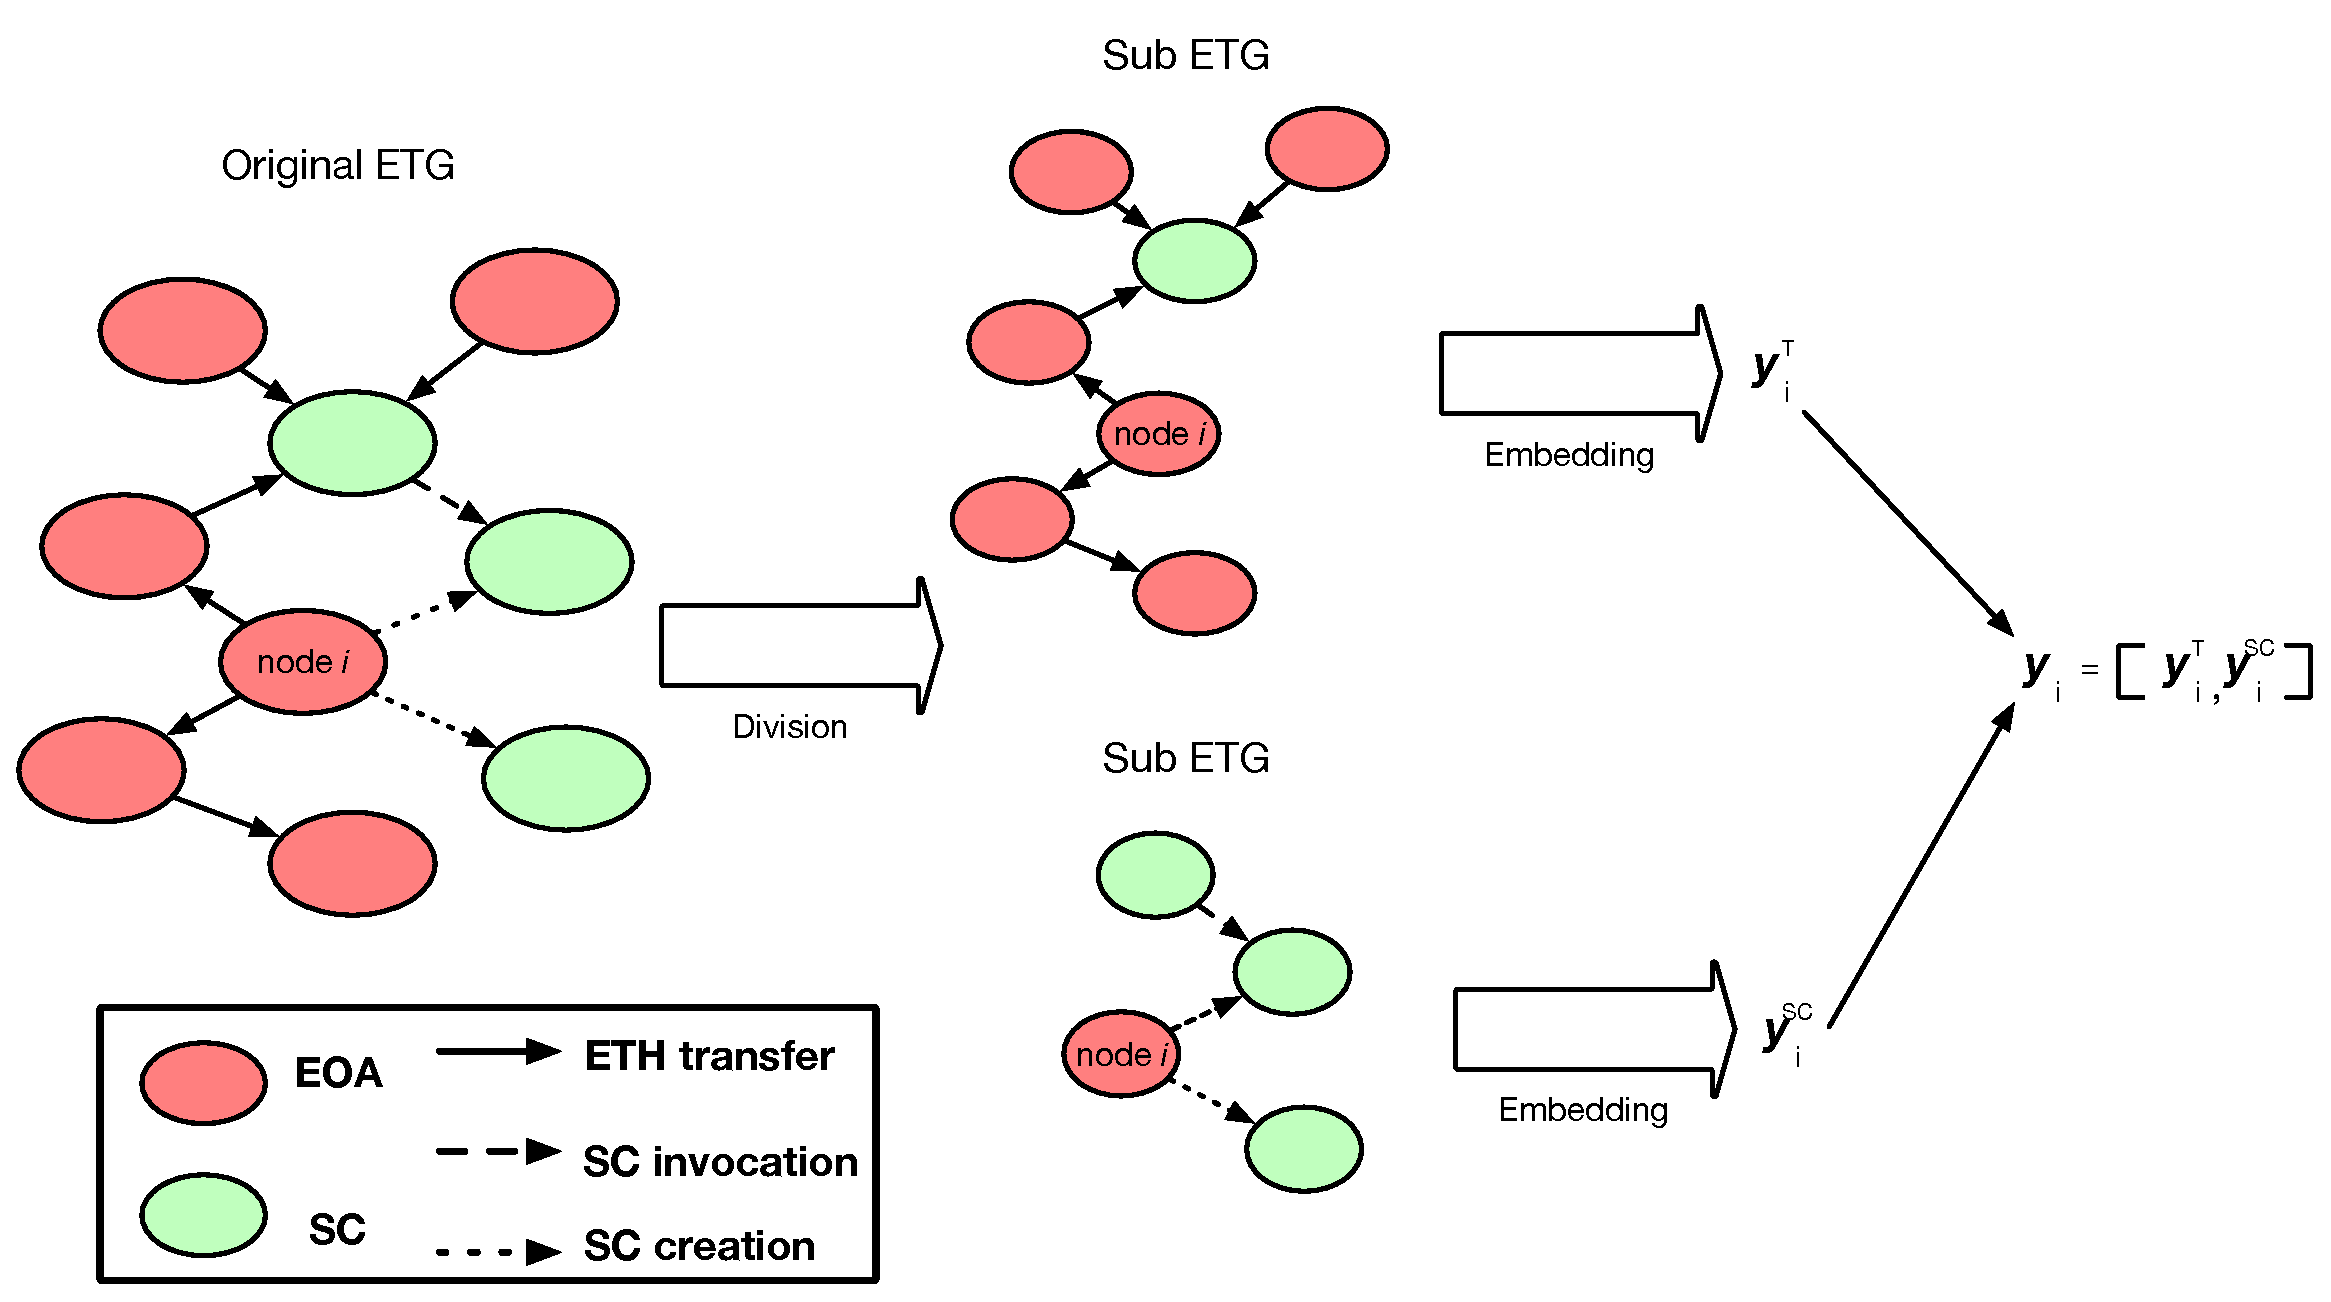
\includegraphics[width=3.5in]{fig/graph_split.eps}
	\caption{Example of a figure caption.}


	%\caption{Example of a figure caption.}
	%\label{fig_graph_split}
\end{figure}

In ETG, edges stand for different activities such as money transfer, contract creation and contract invocation, which can not be measured in a uniform weight model. For example, a weight of assets transfer maybe the ETH amount, however an invocation to smart contract does not have such numerical value. This inspired us to divide the raw ETG into different relation graphs.

%\textbf{Definition 1.} $G^{T}=\{V^T,E^T\}$, where $V^T$ is the subset of $V$. $E^T=\{(v_i,v_j,w)|v_i,v_j \in V^T,w \in \mathbb{R^+}\}$ where an edge $(v_i,v_j)$ indicates that there is at least one ETH transfer from node $v_i$ to $v_j$. And $w$ is the summation of all transferred ETH amount from $v_i$ to $v_j$ for a period of time.

%Actually, $G^T$ represents the ETH trading activities in Ethereum, and each node in $V^T$ has at least one ETH transaction.

%\textbf{Definition 2.} $G^{SC}=\{V^{SC},E^{SC}\}$, where $V^{SC}$ is the subset of $V$. $E^{SC}=\{(v_i,v_j,w)|v_i,v_j \in V^{SC},w \in \mathbb{R^+}\}$ where an edge $(v_i,v_j)$ indicates that there is at least one smart contract creation or invocation from node $v_i$ to $v_j$. And $w$ is the summation of \emph{CREATE} transaction and \emph{CALL} with $0$ ETH transactions for a period of time. 


%And $w$ is the summation of all transferred ETH amount from $v_i$ to $v_j$ for a period of time.

Relational Graph Convolutional Networks (rGCNs) is proposed to develop an encoder model for edges in the relational graph~\cite{schlichtkrull2018modeling}. The propagation model can be expressed as

\begin{equation}
h_i^{(l+1)}=\delta(\sum_{r\in R} \sum_{j \in N_i^r} \frac{1}{c_{i,r}}W_r^{(l)}h_j^{(l)}+W_0^{(l)}h_i^{(l)})
\label{eq:rgcn}
\end{equation}

where $r \in R$ represents a kind of relation ,$N_i^r$ denotes the set of neighbor indices of node $v_i$ under relation $r$, and $c_{i,r}=\frac{1}{|N_i^r|}$. Besides, single self-connection is introduced as a special relation type to each node. %compared with Eq.\ref{eq:gcn}

We divide the edge set into four relations, CALLs with ETH, CALLs without ETH, CREATIONs and REWARDs, according to the their transaction type. Note that the ERC-20 token transfers are categorized as CALLs without ETH which includes normal smart contract invocations as well. The reason is that even though ERC-20 token transfer is a kind of assets transfer intrinsically, it exists in the form of a smart contract in ETG.\footnote{Another reason is that even converting some ERC-20 tokens into ETH is available, the exchange-rate fluctuations make the unification meaningless.} % The reason is that ERC-20 token transfer is a kind of contract invocation and the transaction value is $0$ in an ERC-20 \emph{CALL} transaction.


\subsection{Time-density}
\label{section:time}
Even in a specific relation graph, there are repeated edges between the same node pairs. This occurs quite naturally since an account may transfer or invoke to another account repeatedly.

Note that these activities are located at different time intervals along the time axis which are characterized by the block height. Intuitively, a simple solution is to merge those edges by weight summation but this will lose time information. 

Here we introduce an index\textcolor{red}{?} named time-density which can be represented as strictly increasing function of block height variance.

\begin{equation}
\tau_{ij}^r=g(var(\texttt{bn}_{ij}^r))
\label{eq:time}
\end{equation}

where $\texttt{bn}_{ij}^{r}$ is the block height set of relation $r$ between node $v_i$ and $v_j$. And the new adjacency matrix in relation $r$ can be represented as 

\begin{equation}
\hat{A}=\hat{D}^{-\frac{1}{2}}(\tilde{A}+V)\hat{D}^{-\frac{1}{2}}
\label{eq:?}
\end{equation}

where $V_{ij}=\tau_{ij}$, and $\hat{D}$ is a diagonal matrix where $\hat{D}_{ii}=\sum_{j}(\tilde{A}_{ij}+V_{ij})$.

\textcolor{red}{TBA}

\subsection{High Order and Asymmetric Proximity}
In weighted graph, the edge weight $A_{ij}$ in adjacency matrix $A$ is generally treated as a measure of similarity between nodes $v_i$ and $v_j$. And the higher the edge weight, the more similar the two nodes are expected to be. Edges weight $A_{ij}$ is called \emph{first-order proximity} between nodes $v_i$ and $v_j$. 

Further, \emph{second-order} compares the neighborhood of two nodes and treat them as similar if they have a similar neighborhood~\cite{goyal2018graph}. 

However, in ETG, two nodes are more similar if they have similar connectivity structures instead of they are just connected by an edge with larger weight or share similar neighborhoods. As shown in Figure \ref{fig:high_order}, nodes $v_a$ and $v_c$ are smart contracts and node $v_b$ is normal user. Obviously, $v_a$ is not adjacent to $v_c$  but they have similar neighbor structure. Embedding models with \emph{first-order proximity} and \emph{second-order proximity} will keep them far apart although they have similar connection structures. 

\begin{figure}[htbp]
	\centering
	\subfigure[Example of a high-order proximity caption.]{
		\label{fig:high_order}
		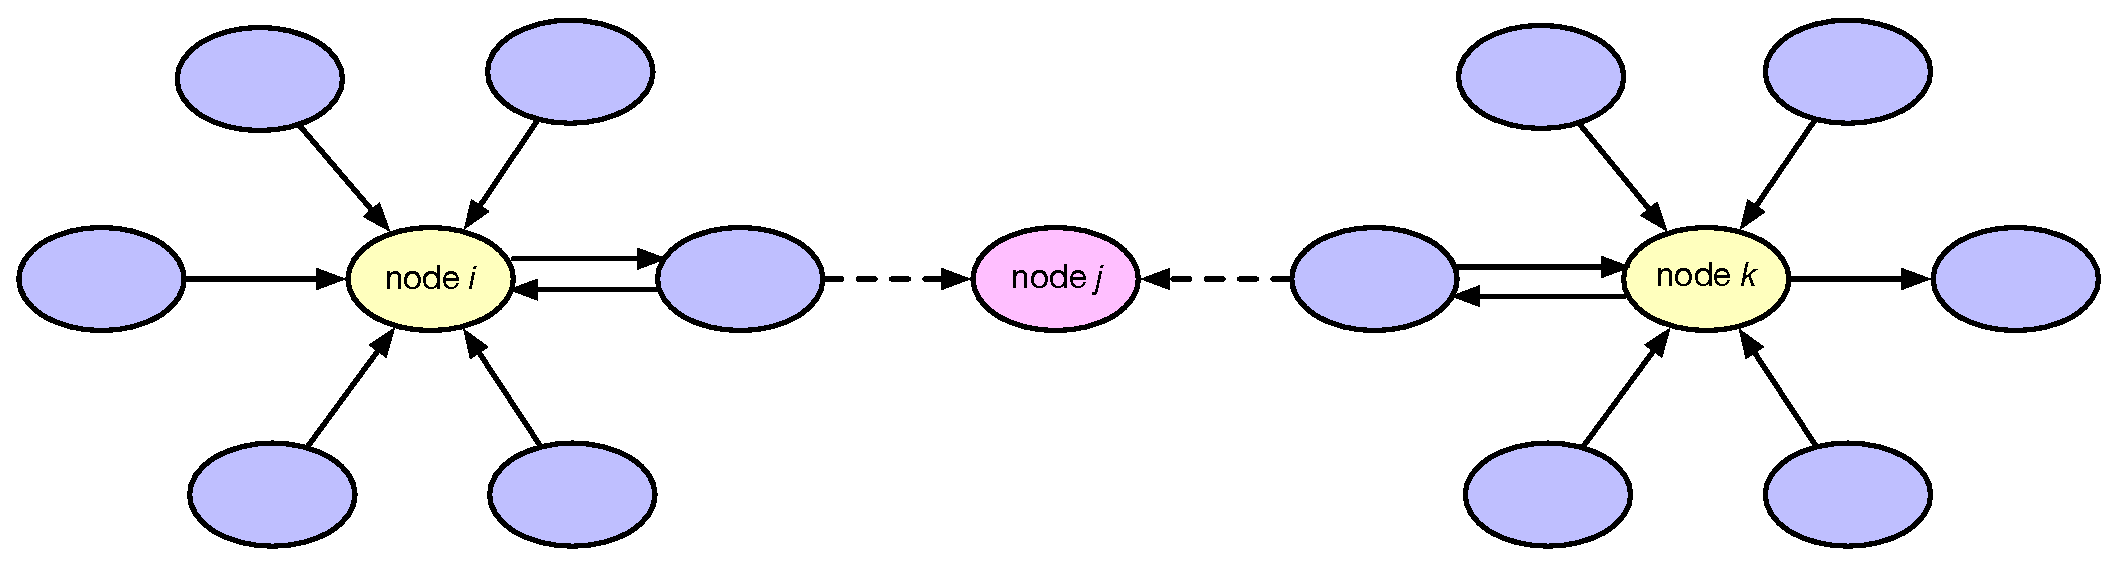
\includegraphics[width=2.0in]{fig/high_order_proximity.eps}
	%\caption{Example of a high-order proximity caption.}
	}
	\subfigure[Example of an asymmetric proximity caption.]{
		\label{fig:asymmetric}
		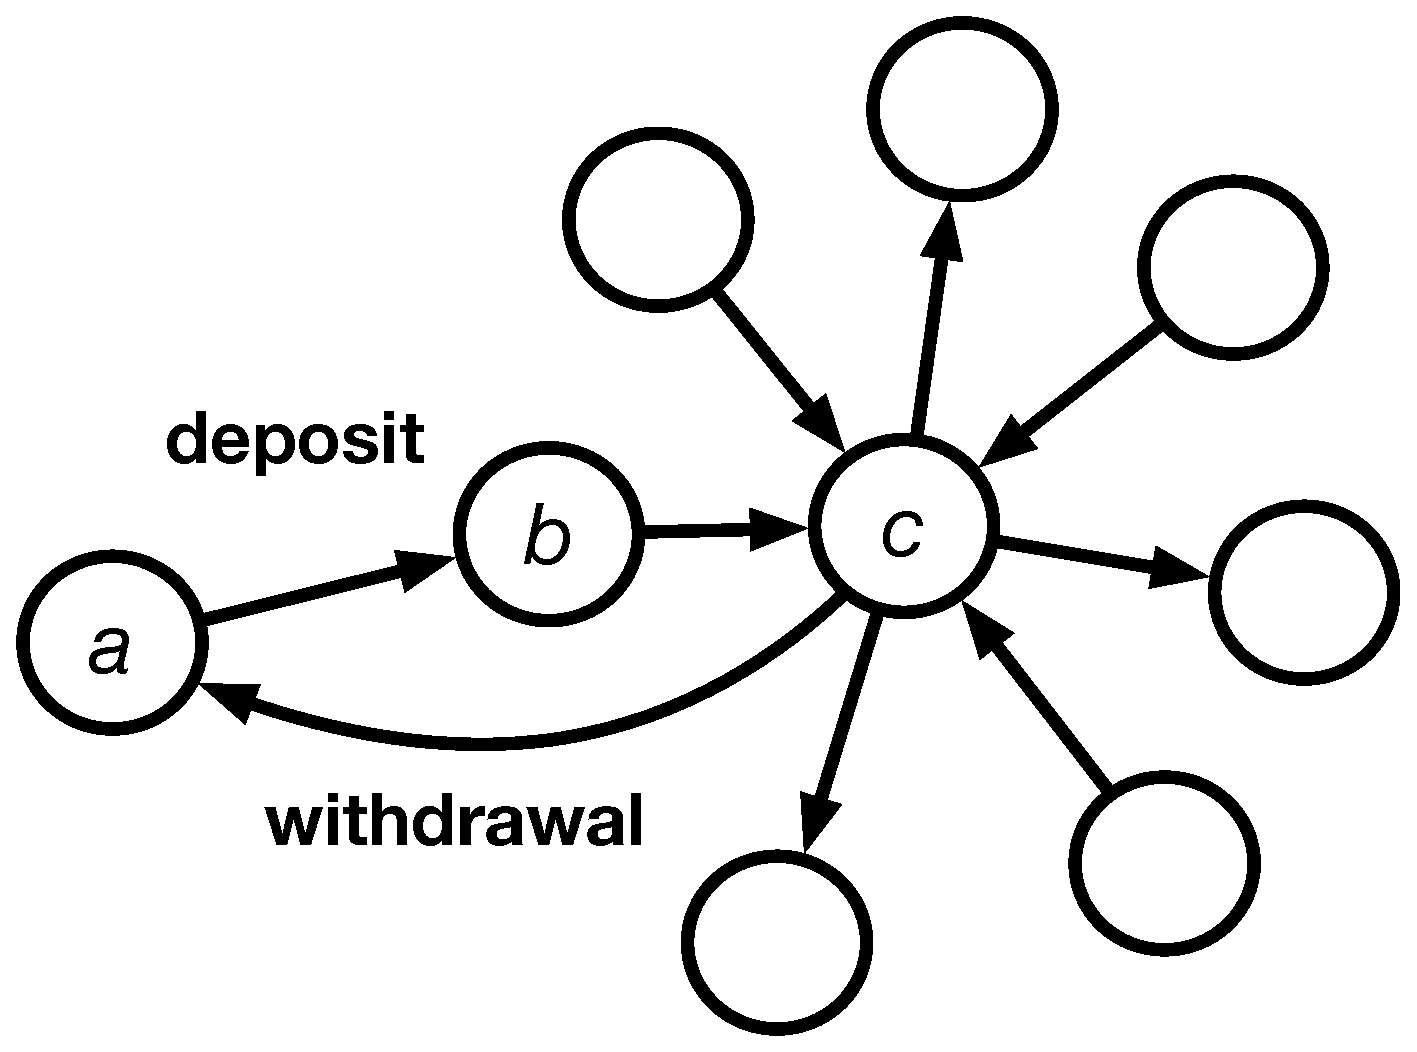
\includegraphics[width=1.5in]{fig/asymmetric.eps}
	}
	\caption{Examples of an asymmetric proximity.}

\end{figure}

To preserve higher order proximities, the hidden layer number in our model is set as 2.

\textcolor{red}{TBA This is second order proximity.}

Another property of closeness in ETG is \emph{asymmetric proximity}. For instance, as shown in Figure. \ref{fig:asymmetric}, node $v_a$ is a Ethereum investor address and node $v_c$ is an exchange root address. Generally, edge weight can be $A_{ab}=A_{bc}=A_{ca}$ since deposit and withdrawal come in pairs in symmetric model. However, the proximity $(v_a,v_c)$is not equal with proximity $(v_c,v_a)$ due to their asymmetric local structures.


 Zhou et. proposed a scalable asymmetric proximity preserving graph embedding method based on random walk~\cite{zhou2017scalable}. In their model, the probability that $v_a$ arrives at $v_c$ is far less than the one that $v_c$ arrives at $v_a$, due to their asymmetric local structures. However, there is no research on asymmetric proximity in GCN model.
 
 To preserve asymmetric proximity, we..
 
 \textcolor{red}{TBA.}


% !TEX root = main.tex

\section{XXX Model}
To address the above-described challenges, we illustrate XXX, which is first approach~\textcolor{red}{(or system?)} for cryptocurrency transaction graph analysis based on graph embedding.

Fig.~\ref{fig:architecture} depicts the overall architecture of our XXX model. Correlating to the three phases introduced in section~\ref{subsec:methodology}, we explain our model in following three aspects, \emph{preprocessing}, \emph{embedding} and \emph{prediction}.

\begin{figure}[htbp]
	\centering
	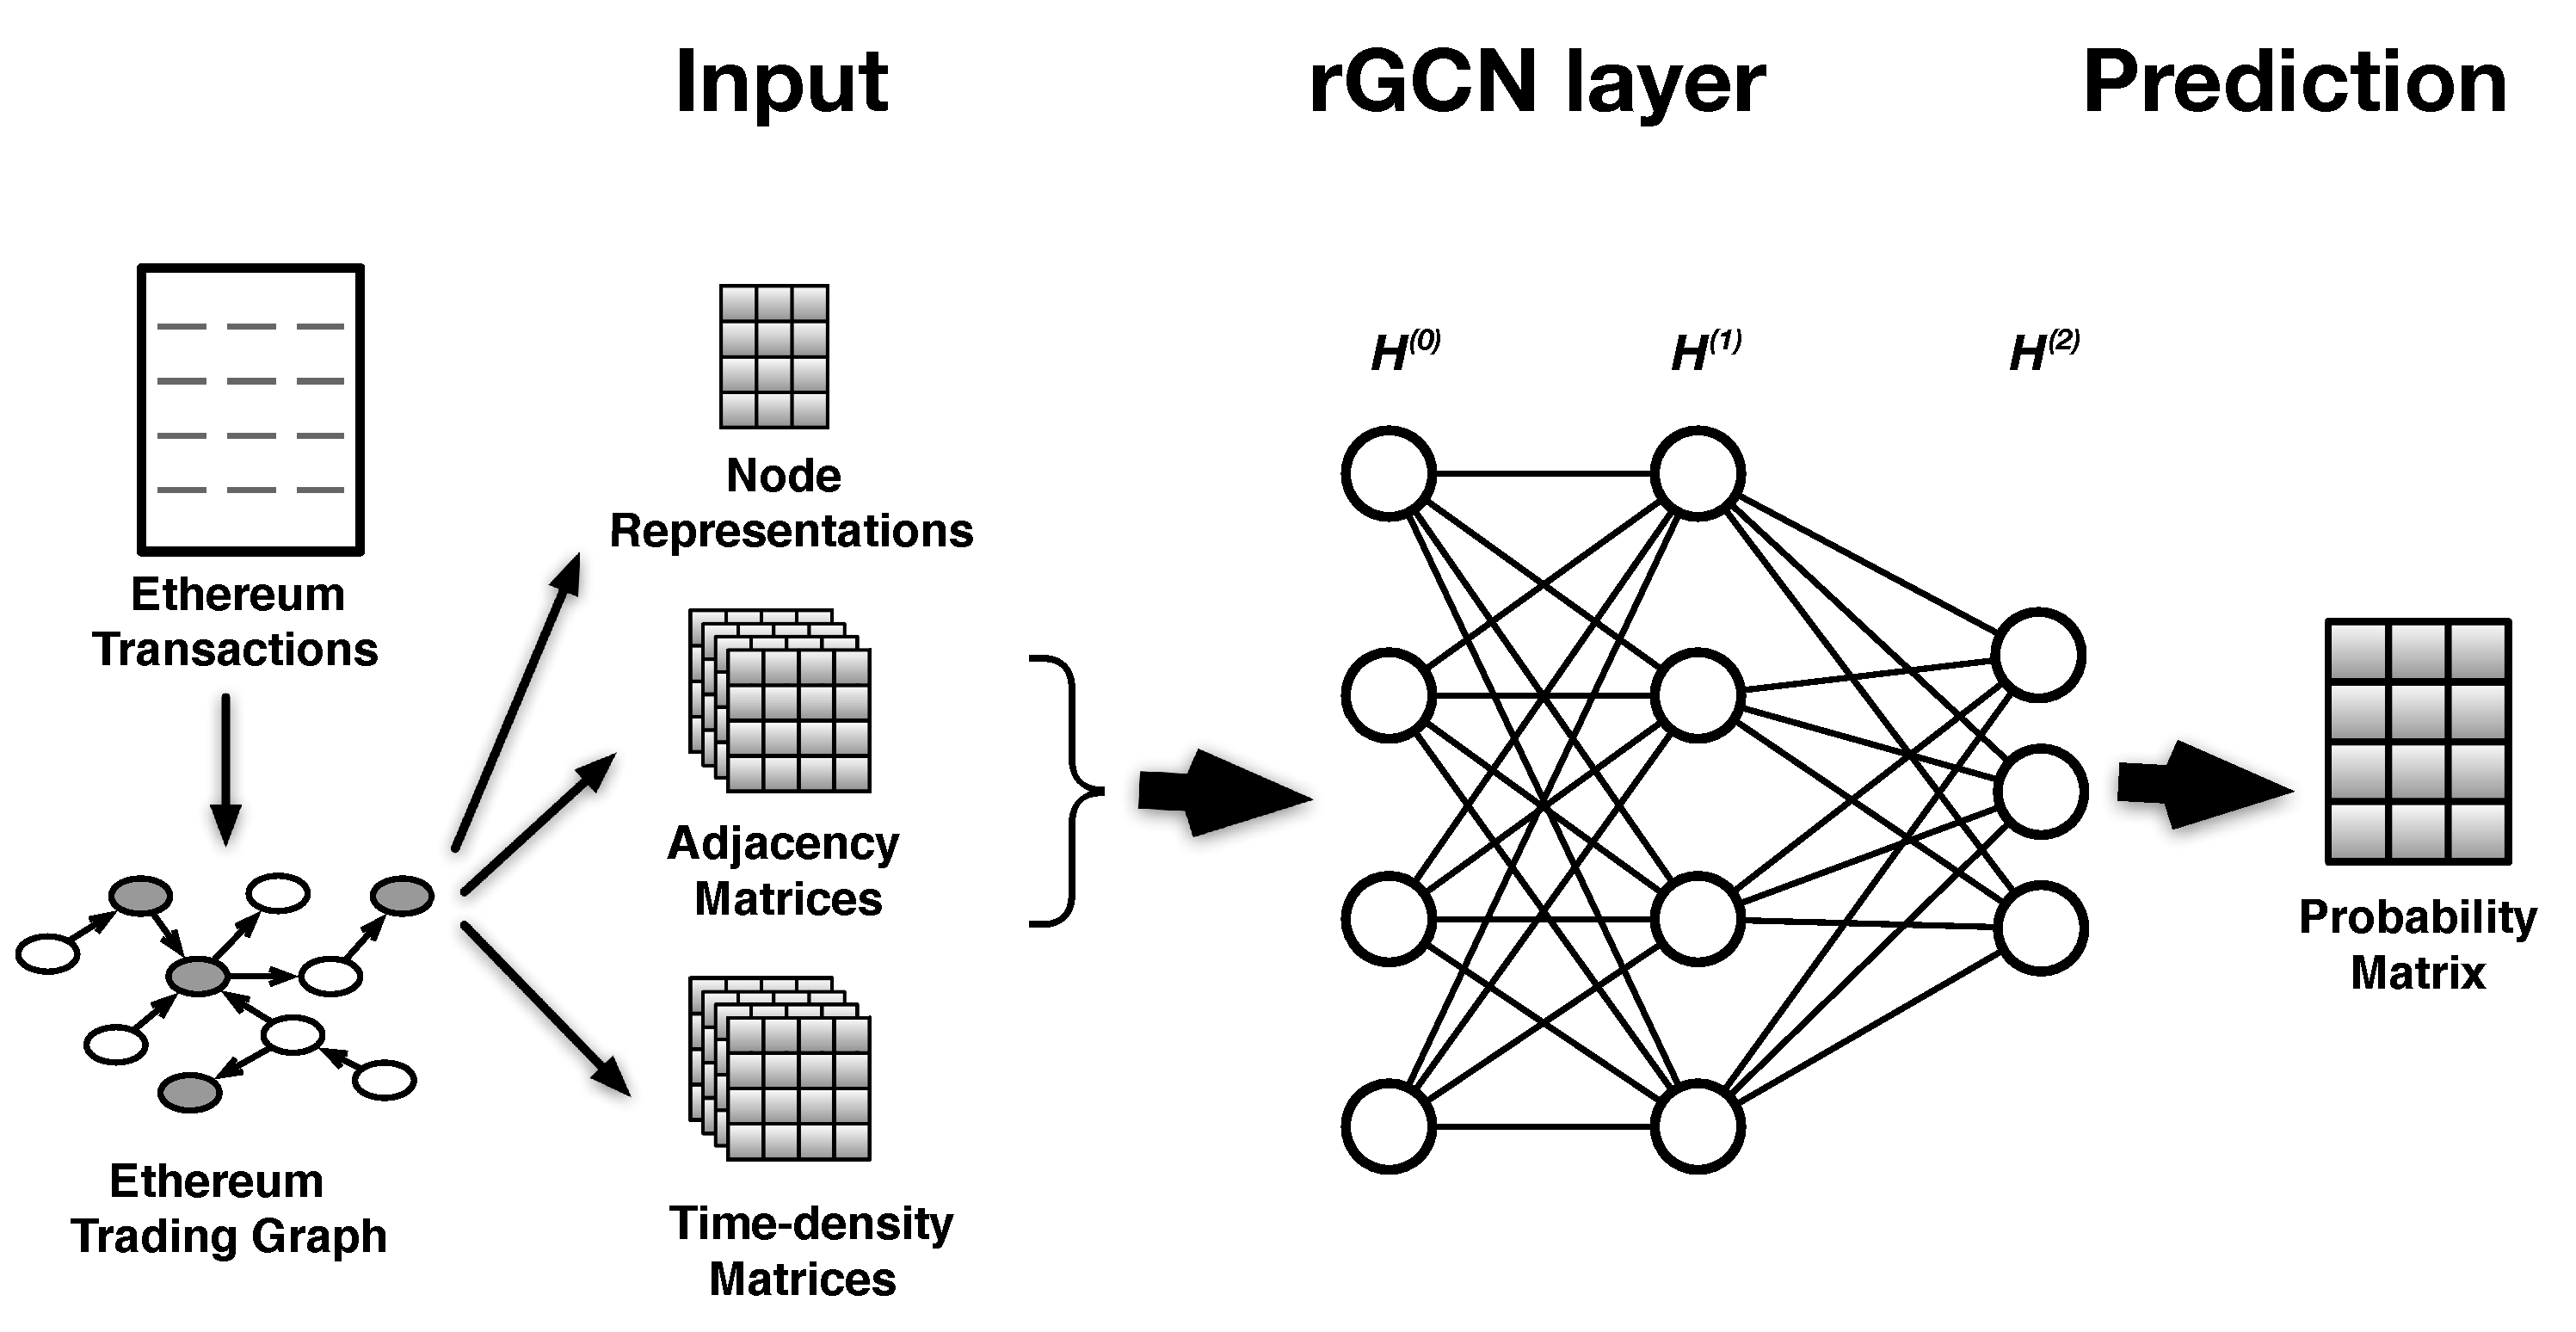
\includegraphics[width=3.5in]{fig/architecture.eps}
	\caption{Overall architecture.}
	\label{fig:architecture}
\end{figure}


\subsection{Preprocessing}
\label{sec:input}
In the preprocessing, the Ethereum transaction graph is constructed based on original transaction logs at first. Different from other studies, the graph is translated to several matrices as the input of embedding model.

 The inputs consist of three parts: (1) a node representation matrix that captures the structural and additional information of accounts, (2) a list of adjacency matrices which describe different relations, and (3) a list of time-density matrices that represent transaction intensiveness between each pair of nodes.

\textbf{Account representations.} We use a feature matrix $X \in \mathbb{R}^{N \times d}$ to encode the overall structural and additional information of each account. The $d$ terms include some pre-defined vectors and here we use the following features
\begin{itemize}
	\item \emph{in-degree}: the number of edges incoming to a node, that is, the number of transactions initialed by an account.
	\item \emph{out-degree}: the number of edges outgoing from a node, that is, the number of transactions which point to an account.
	\item \emph{weighted in-degree}: the summation of all weights of edges incoming to a node, which represents the total Eth received by an account. 
	\item \emph{weighted out-degree}: the summation of all weights of edges outgoing to a node, which represents the total Eth send from an account. 
	%\item eccentricity
	%\item clustering coefficient
	\item \emph{account type}: whether the account is a contract or EOA.
\end{itemize}

%such as in-degree, out-degree, weighted degree, eccentricity, clustering coefficient. Besides, the account type (EOA or SC) is also considered.   

These features help the following layers to pay attention to structural similarity between nodes.

\textbf{Relations.} To investigate the multi-relations in ETG, we divide the raw ETG into different graphs and capture the relations of graph neighboring nodes using adjacency matrices. 

The list of adjacency matrices, $\{A^1,A^2,\dots,A^R|A^i\in \mathbb{R}^{N \times N}\}$ describes the $R$ relations among $N$ nodes in ETG. As we mentioned before, the strategy of division has a large influence on classification performance. 

In our model, the relations are constructed from four categories, including \texttt{CALL} with ETH, \texttt{CALL} without ETH, \texttt{CREATION} and \texttt{REWARD}, which represent the relations of ETH transferring, smart contract invocation, smart contract deployment and mining rewarding. 

We consider the 4 types of forward transactions introduced above and 4 reverse relations in order to pass information from the opposite direction. Besides, a self loop as a special relation type is included to retain information of the previous layer in the GCN network. 

For contract invocation, contract deployment and mining rewarding relations, we calculate the frequency of repeated edges between a nodes pair as the adjacent weight in the corresponding relation adjacency matrix. For ETH transferring, on the other hand, it is not sensible to use the amount of ETH flow directly as the adjacent weight. That is because the accounts have varied enormously in terms of ETH transferring which \textcolor{red}{will lead to underflow and overflow in the process of training.} Here the amount of ETH transferring is discretized into (1) small transfers which the transaction value is less than 1 ETH; (2) medium transfers which the transaction value is between 1 ETH and 10 ETH and (3) major transfers which the transaction value is above 10 ETH. Then the ETH transferring matrix can be calculate as well as the former relations.

Specially, the adjacency matrices are modified to preserve the asymmetric proximity of ETG, which will be addressed in detail later. 

\textbf{Time-density matrices.} We also find that the relationship between a pair of nodes differs from another, even they have the same transaction frequency or adjacency weight. This insight inspire us to use time-density information.

Correlated to the adjacency matrices, a list of time-density matrices $\{K^1,K^2,\dots,K^R|K^i\in \mathbb{R}^{N \times N}\}$ describes the concentration of relations. 

Given a sequence $\{h_{ij1}^r,h_{ij2}^r,\dots,h_{ijm}^r | h_{ijk}^r>0\}$ as the block height of transactions in relation $r$ between node $v_i$ and $v_j$. The time-density of each relation $r$ is computed as%Equation \ref{eq:time}

\begin{equation}
k_{ij}^r=g(\sqrt{Var[\frac{1}{m}\sum_{k=1}^m h_{ijk}^r]})
\label{eq:time}
\end{equation}

\noindent where $g(\cdot)$ is the function of squash which can be logarithmic function.

\subsection{Embedding}
\label{sec:rGCN layers}
 We feed the input into GCN based model with 2 hidden layers, as a trade-off between preserving high-order proximities and introducing noise.

The input to rGCN $l$-th layer is defined as $H^{(l)}={h_1^{(l)},h_2^{(l)},...,h_N^{(l)}|h_i^{(l)}\in \mathbb{R}^{N \times d^{(l)}}}$.

%In raw rGCN model, the propagation model can be expressed as
%\begin{equation}
%h_i^{(l+1)}=\delta(\sum_{r\in R} \sum_{j \in N_i^r} \frac{1}{c_{i,r}}W_r^{(l)}h_j^{(l)}+W_0^{(l)}h_i^{(l)})
%\label{eq:rgcn}
%\end{equation}
%\noindent where $r \in R$ represents a kind of relation, $N_i^r$ denotes the set of neighbor indices of node $v_i$ under relation $r$, and $c_{i,r}=\frac{1}{|N_i^r|}$. Single self-connection is also introduced as a special relation type to each node. %compared with Eq.\ref{eq:gcn}The node feature $h_i$ is updated as:

To 

We modified the forward updating process as 
\begin{equation}
h_i^{(l+1)}=\delta(\sum_{r\in R} \sum_{j \in N_i^r} \frac{\tau_{ij}^r}{\hat c_{i,r}}W_r^{(l)}h_j^{(l)})
\end{equation}

\noindent where $\tau_{ij}^r$ is the time-density of transactions from node $v_i$ to $v_j$. 

The coefficient $\hat c_{i,r}$ is computed as:
\begin{equation}
\hat c_{i,r}=\frac{1}{d_i^r\cdot N_i^r}
\end{equation}

\noindent where $d_i^r=\sum_{j}A^r_{ij}$, preserving the asymmetric proximity.


\subsection{Prediction and Training}
The output of the last layer indicates the probability that each point being assigned to each class.

The output of the last rGCN layer is regarded as a probability matrix $P=\{p_1,p_2,...,p_N|p_i\in \mathbb{R}^{N \times m}\}$, where $p_i=\{p_{i,1},p_{i,2},...,p_{i,m}\}$ describes the probability of classifying node $v_i$ into $m$ categories. 

We utilize the cross-entropy loss function as the training objective:
\begin{equation}
L=-\sum_{i=1}^T\sum_{j=1}^m y_{i,j}\log p_{i,j}+\lambda ||\theta||^2
\end{equation}

\noindent where $T$ is the number of training samples, $y_{i,j}$ is the true probability of node $v_i$ belonging to category $j$. $\theta$ is the set of all parameters and $\lambda$ is the coefficient for $L_2$  regularization.


\bibliography{reference}

\end{document}

%%% Local Variables:
%%% mode: latex
%%% TeX-master: t
%%% End:
